%preamble
\documentclass[letterpaper]{article}
\synctex=1
\usepackage{graphicx}
\graphicspath{ {images/} }

\usepackage{lipsum}
\usepackage{float}
% \bibliographystyle{IEEEtran}
% \bibliographystyle{ieeetr}

\usepackage{amssymb}

\usepackage{siunitx}

\usepackage{multirow}
% for merging table cells I think

\usepackage{tabularx}
% allows for linewrap within cells
\newcolumntype{Y}{>{\centering\arraybackslash}X}

\usepackage{todonotes}

% \usepackage[utf8]{inputenc}
% \usepackage[russian]{babel}
% WHY CAN'T I USE є IN MATH MODE
% \usepackage[T2A,T1]{fontenc}
% \DeclareSymbolFont{cyrillic}{T2A}{cmr}{m}{n}
% \DeclareMathSymbol{\Sha}{\mathalpha}{cyrillic}{216}
% \DeclareMathSymbol{\cyrje}{\LastDeclaredEncoding}{106}

\usepackage{fancyhdr} %header
\fancyhf{}
\fancyhead[R]{Arun Woosaree XXXXXXX}
\renewcommand\headrulewidth{0pt}
\fancyfoot[C]{\thepage}
\renewcommand\footrulewidth{0pt}
\pagestyle{fancy}

% make subsection use letters
\renewcommand{\thesubsection}{\thesection\ \alph{subsection})}


% \usepackage{amsthm}

%actual document
\begin{document}

% \maketitle %insert titlepage here
\begin{titlepage}
 \begin{center}
  \vspace*{1cm}
  \Huge
  Stat 235
  \vspace{1cm}
  
  Lab 5
  \vspace{1cm}
  
  WOOSAREE, Arun
  \vspace{1cm}
  
  \Huge
  Lab EL12
  \vspace{1cm}
  
  TA: Jessa Marley
  \vspace{1cm}
  
  \today
  \vfill
 \end{center}
\end{titlepage}

\section{}
\label{q1}

\subsection{}
% OUTPUT: 3 Scatterplots, thrust vs. Fuel flow rate, thrust vs.
% exhaust temperature, thrust vs. Ambient temperature.
% What should be on the y-axis?
\todo{captions}
\begin{figure}[H]
 \centering
 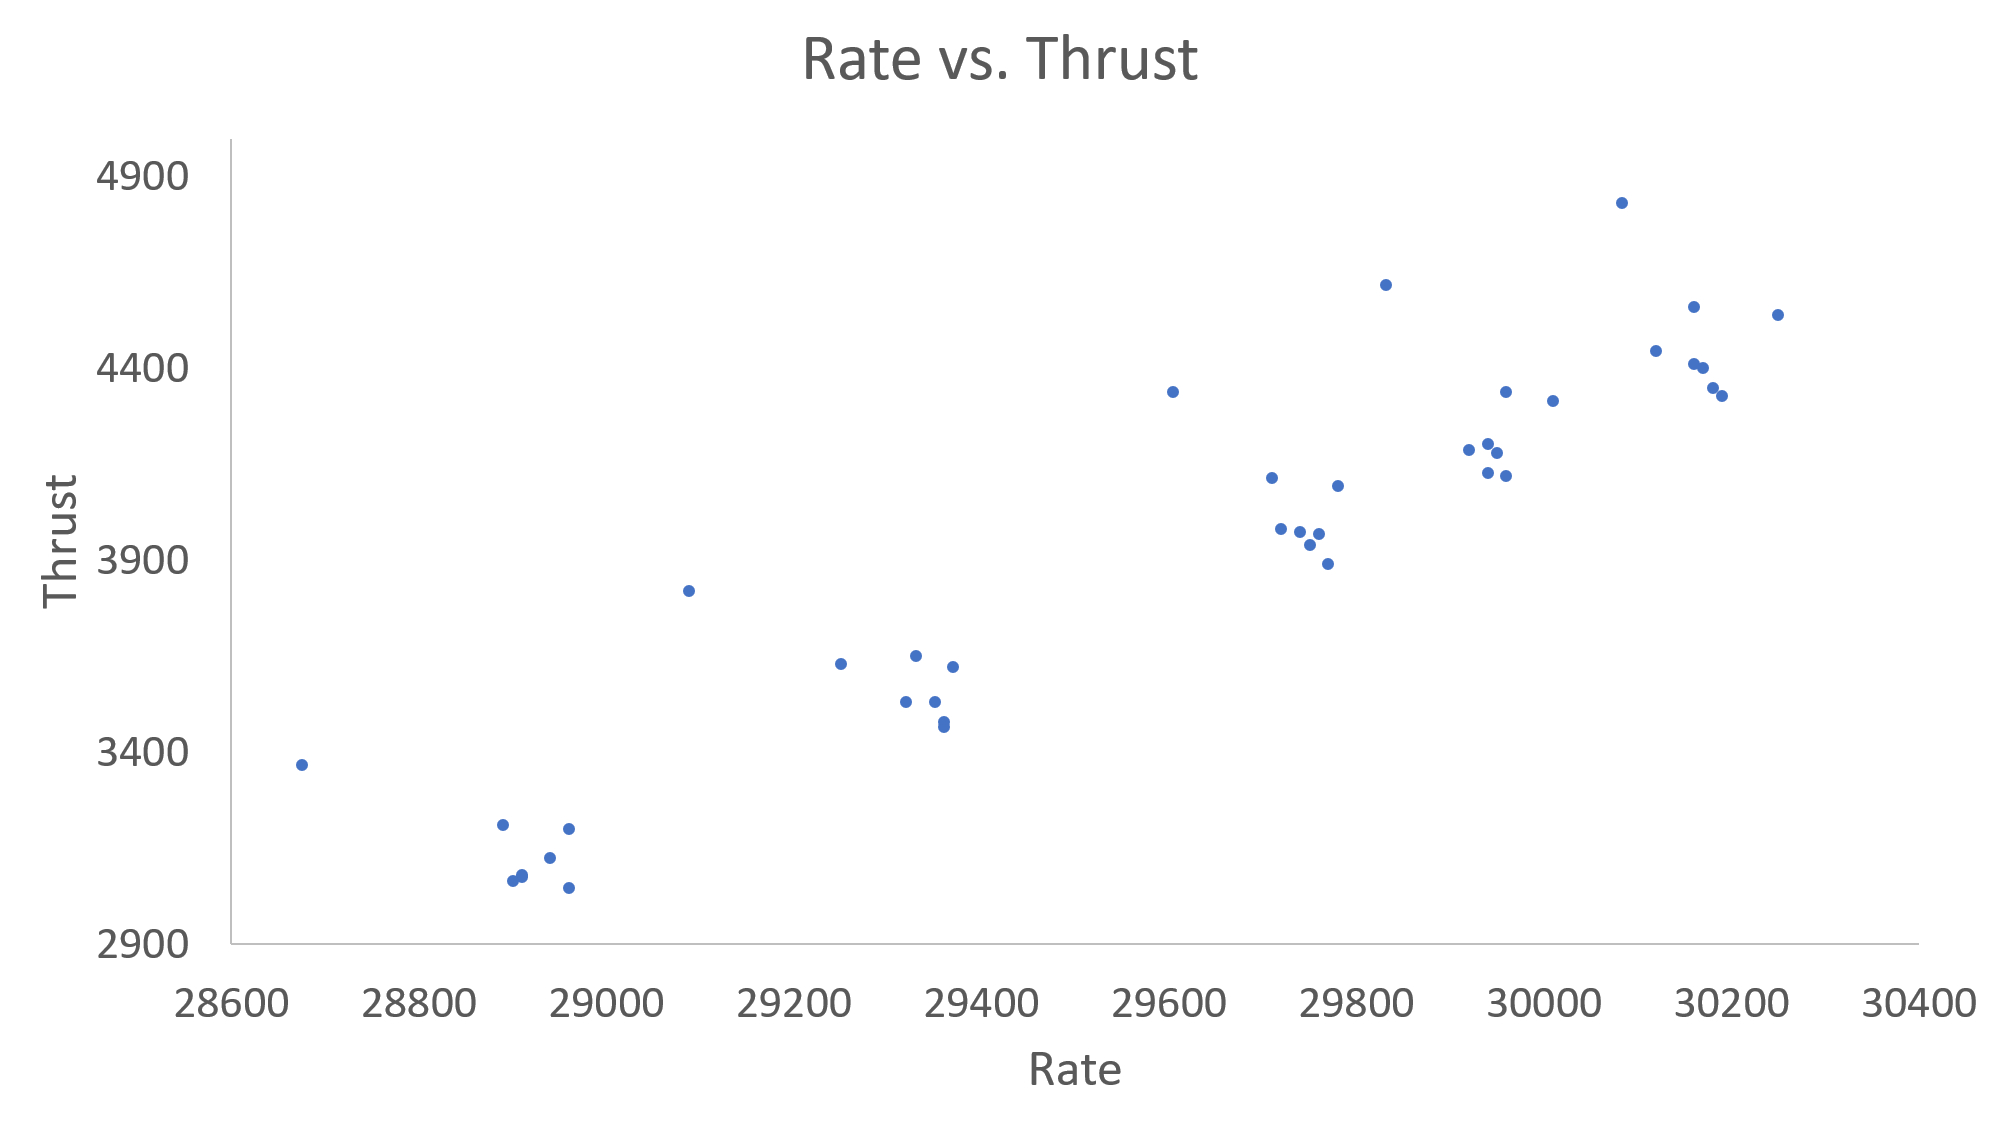
\includegraphics[width=\textwidth]{ratethrust.png}
 \caption{INSERT CAPTION HERE}
 \label{ratethrust}
\end{figure}

\begin{figure}[H]
 \centering
 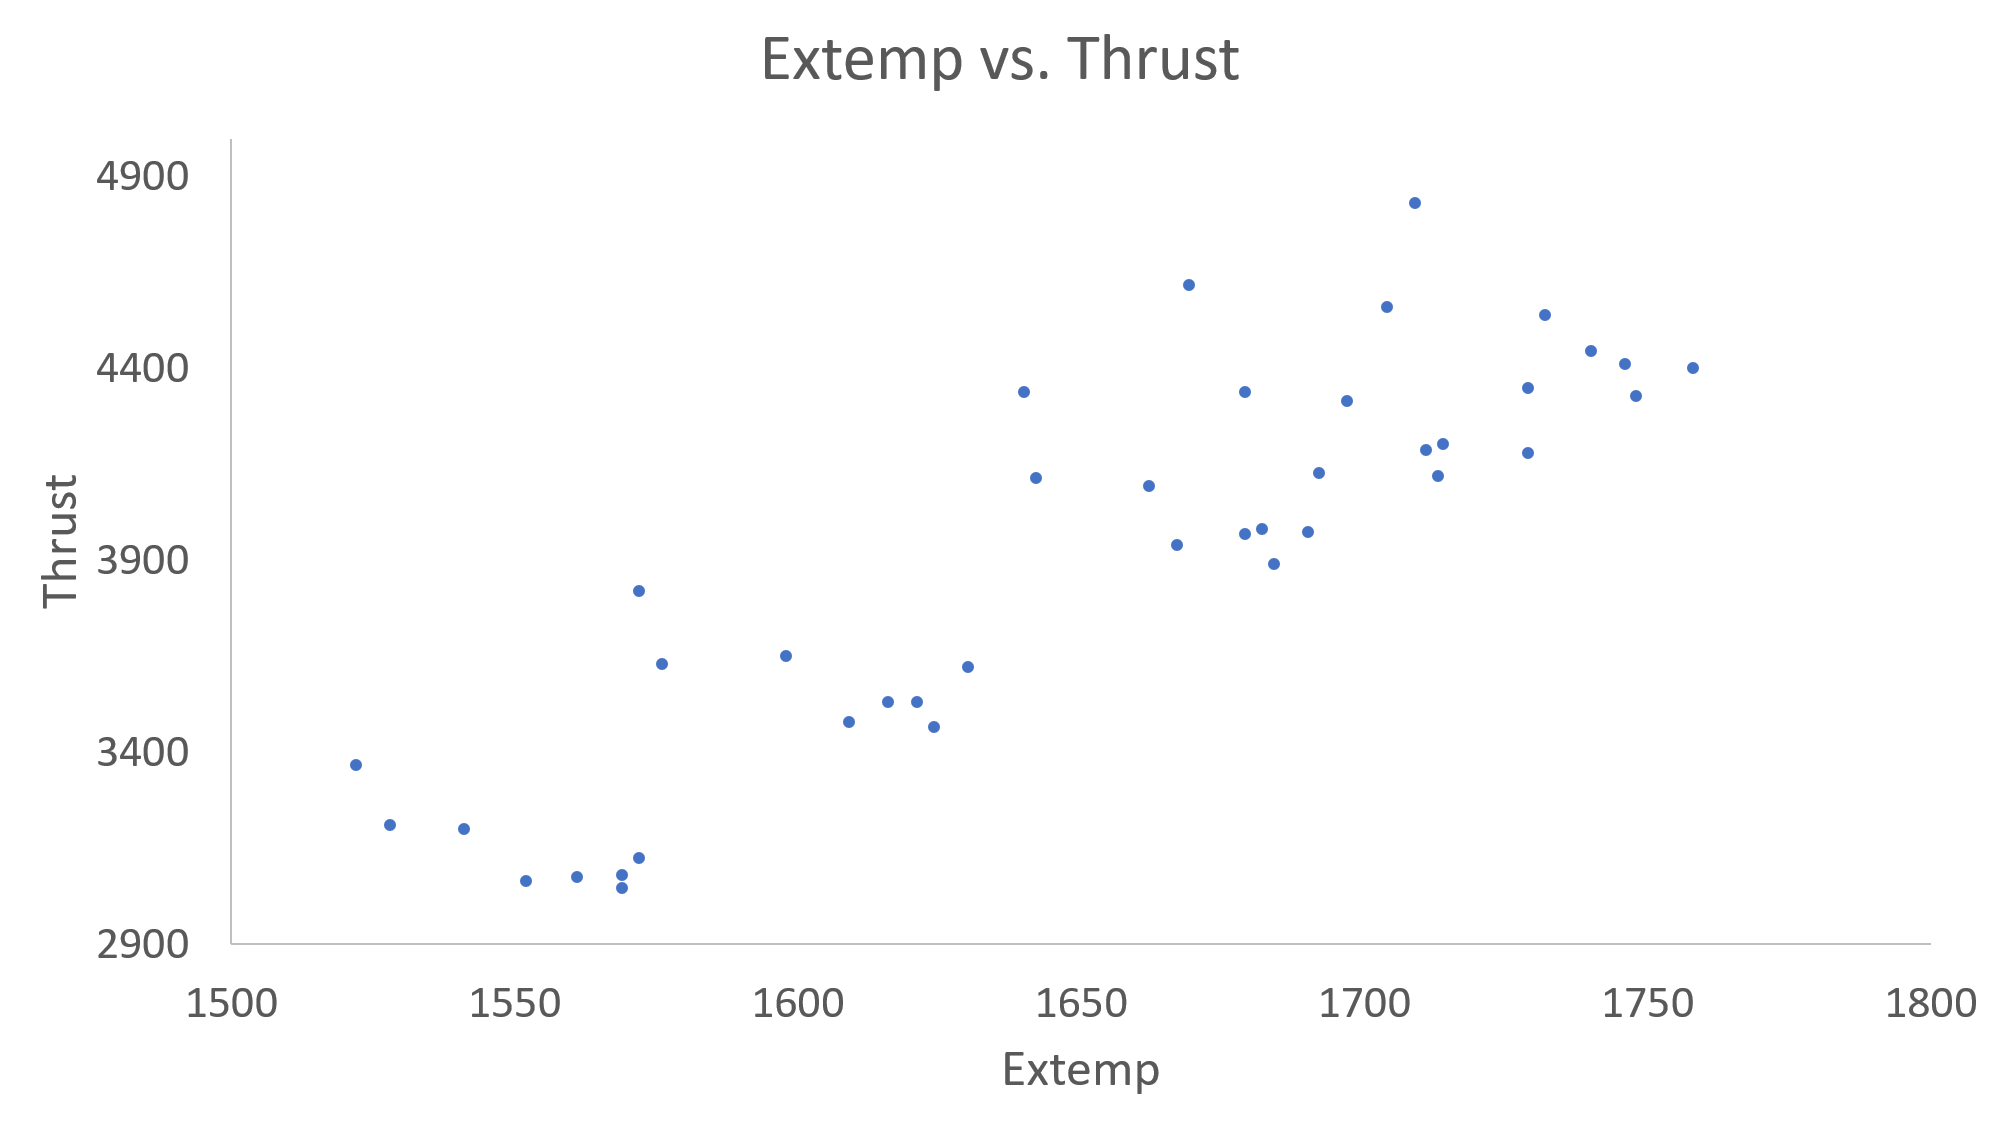
\includegraphics[width=\textwidth]{extempthrust.png}
 \caption{INSERT CAPTION}
 % \label{q6}
\end{figure}

\begin{figure}[H]
 \centering
 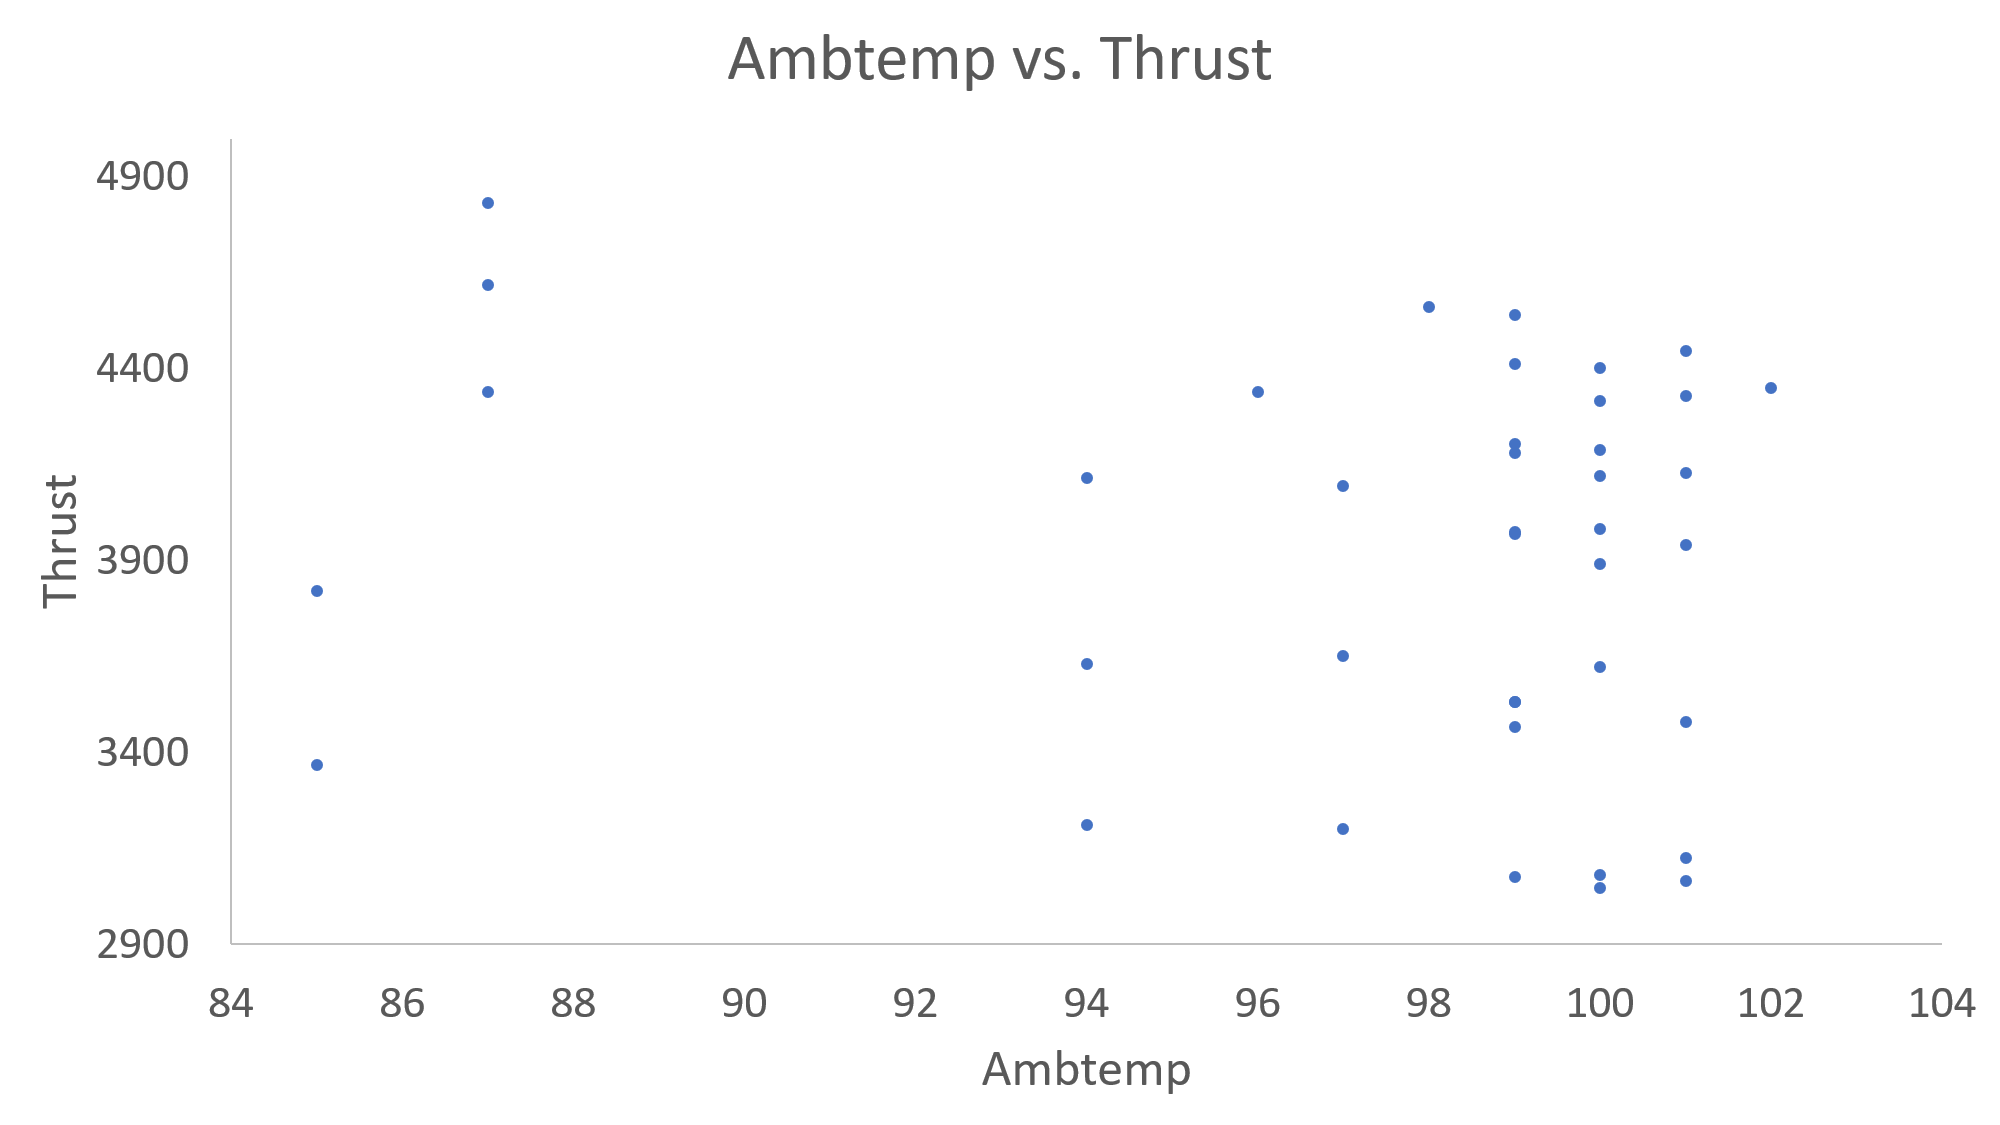
\includegraphics[width=\textwidth]{ambtempthrust.png}
 \caption{INSERT}
 % \label{q6}
\end{figure}

\subsection{}
\label{1b}
% Look at the center of the “clouds”.  Are they linear? Strength of
% linear relationship?

\begin{itemize}
 \item The plot for rate vs. thrust above appears to exhibit a relatively strong positive
       linear relationship, with less scatter relative to the other plots.
 \item The plot for extemp vs. thrust above appears to exhibit a fairly strong positive
       linear relationship, but with a bit more scatter than Figure \ref{ratethrust}.
 \item The plot for ambtemp vs. thrust above does not appear to exhibit a strong linear
       relationship due to the points being very visually scattered.
       If there is a linear relationship, it looks like it would be almost flat,
       with a slightly negative slope.
\end{itemize}

Overall, the rate seems to have the stongest linear relationship with the thrust,
since it has a positive slope and the least amount of scatter.
\todo{Which of the three predictor variables seems to be the best predictor of thrust?}
So it's the best predictor?

\section{}

\subsection{}
% OUTPUT: Correlation matrix.

\begin{table}[H]
 \centering
 \begin{tabular}{c|c|c|c|c|}
          & rate        & extemp      & ambtemp  & thrust \\ \hline
  rate    & 1           &             &          &        \\ \hline
  extemp  & 0.975750317 & 1           &          &        \\ \hline
  ambtemp & 0.216465939 & 0.301764125 & 1        &        \\ \hline
  thrust  & 0.928792499 & 0.87169251  & -0.14744 & 1      \\ \hline
 \end{tabular}
 \caption{Correlation matrix}
 \label{correlationmatrix}
\end{table}
\todo{caption}

\subsection{}
% Highest correlation, lowest (note absolute value)? Does this
% match the conclusions from Q1?

The regressor variable with the largest magnitude of correlation with the response
variable thrust is the rate, with a value of $0.928792499$.
The regressor variable with the lowest magnitude of correlation with the thrust
is ambtemp, with a value of $-0.14744$.
The values obtained in Table \ref{correlationmatrix} agree
with the conclusions reached in Question \ref{q1}, with
the rate having the largest correlation with a positive slope, and the
ambient temperature having a weak correlation and slightly negative slope.
Additionally, we see that the external temperature also has a fairly strong
linear relation with the thrust, and its correlation value is both positive and less than
the rate variable, as predicted in Question \ref{1b}.
\todo{maybe be more precise}

\section{}
% Define the model as an equation, use the basic equation of
% regression. Assumptions of regression?

The regression model is as follows:
\begin{equation}
 y = \beta_0 + \beta_1 x + \epsilon
 \label{model}
\end{equation}
, where $y$ is the thrust, $x$ is the fuel flow rate, $\beta_0$ is the y-intercept, $\beta_1$
is the slope, and $\epsilon$ is the random error.
The model's assumptions are as follows:
\begin{itemize}
 \item The distribution of $\epsilon$ at any $x$ has a mean of 0 ($\mu_\epsilon=0$ to aid linearity)
 \item The standard deviation of $\epsilon$ is the same for any $x$ (it's constant)
 \item The distribution of $\epsilon$ at any $x$ is normal
 \item The random deviations $\epsilon_1, \epsilon_2, ..., \epsilon_n$ associated with different observations are independent of one another
\end{itemize}

\section{}
% OUTPUT: Regression output from excel, not necessary/being marked.

\subsection{}
% Equation of regression with coefficient values. Determine
% influential points from scatter plot in Q1. Determine outlier residuals from residual plot.

Using the regression tool in Excel, we find $\beta_0=-25860.12772$, and
$\beta_1=1.005348711$.
So, Equation \ref{model} becomes
$$ thrust = -25860.12772 + 1.005348711 \times (rate) + \epsilon$$
\todo{should $\epsilon$ be in this equation?}

The following points from the scatterplot in Figure \ref{ratethrust} were visually far
away from the rest of the data, and are therefore influential on the fitted line:
\begin{itemize}
 \item[] (rate, thrust)
 \item[] (28675, 3368),
 \item[] (29088, 3820),
 \item[] (29604, 4340),
 \item[] (29831, 4617), and
 \item[] (30083, 4833)
\end{itemize}

The following points on the residual plot had relatively large residuals which were
visually far away from the rest of the data:
\begin{itemize}
 \item[] (rate, residual)
 \item[] (28675, 399.7534461),
 \item[] (29088, 436.5444286),
 \item[] (29604, 437.784494),
 \item[] (29831, 486.5703367), and
 \item[] (30083, 449.2224616)
\end{itemize}

\subsection{}
The estimate of the model standard deviation is:
$$s = 189.466735$$
\todo{compare to average? wtf???}

\subsection{}
% Percent of variation? What might explain variation?

The percentage of the variation in thrust which is explained by the fuel flow rate
is the $R^2$ value.
$$R^2 = 0.862655506 \approx 86.27\%$$
The other predictor variables extemp and ambtemp may explain the remaining variation
(probably the extemp variable moreso than the ambtemp variable).
% \todo{What other possible predictor variables may explain the remaining variation?}

\subsection{}
% Hypotheses? What kind of test can you use? Values of test
% statistics? P-value? Null distribution? Conclusion?

Let the null hypothesis be that the fuel flow rate does not have any value in explaining the thrust:
$$ H_0: \beta_1 =0 \quad vs. \quad H_A: \beta_1 \neq 0 $$
The distribution of the test statistic follows a null dustribution.
Using Excel, we find that
$$F_0 = 0.586694336 \sim F_{39-2}^{1}$$
\todo{idk what I'm doing wrong here}
The p-value is
$$p= \SI{5.72762e-18}{} $$

Because the p-value obtained is extremely small, we reject $H_0$. i.e. the data strongly suggests that there is a relationship between the fuel flow rate and the thrust.

\subsection{}
The mean change in thrust as the fuel flow rate increases by 1 unit is the slope.
From the Regression Tool output, we find that the 95\% confidence interval
for this is:
$$(0.873611965, 1.137085456)$$

\subsection{}
% Predicted value? Residual?

With a flow rate of 30 250, the predicted thrust is:
$$\hat{y} = \hat{\beta_0} + \hat{\beta_1}x = -25860.12772 + 1.005348711 \times 30250 \approx 4551.671 $$
In this case, the value of the residual is
$$e = y-\hat{y} = 4540 - 4551.671 = -11.67077$$

\subsection{}
% OUTPUT: Residual plot. Interpret the plot, are the assumptions met?

\begin{figure}[H]
 \centering
 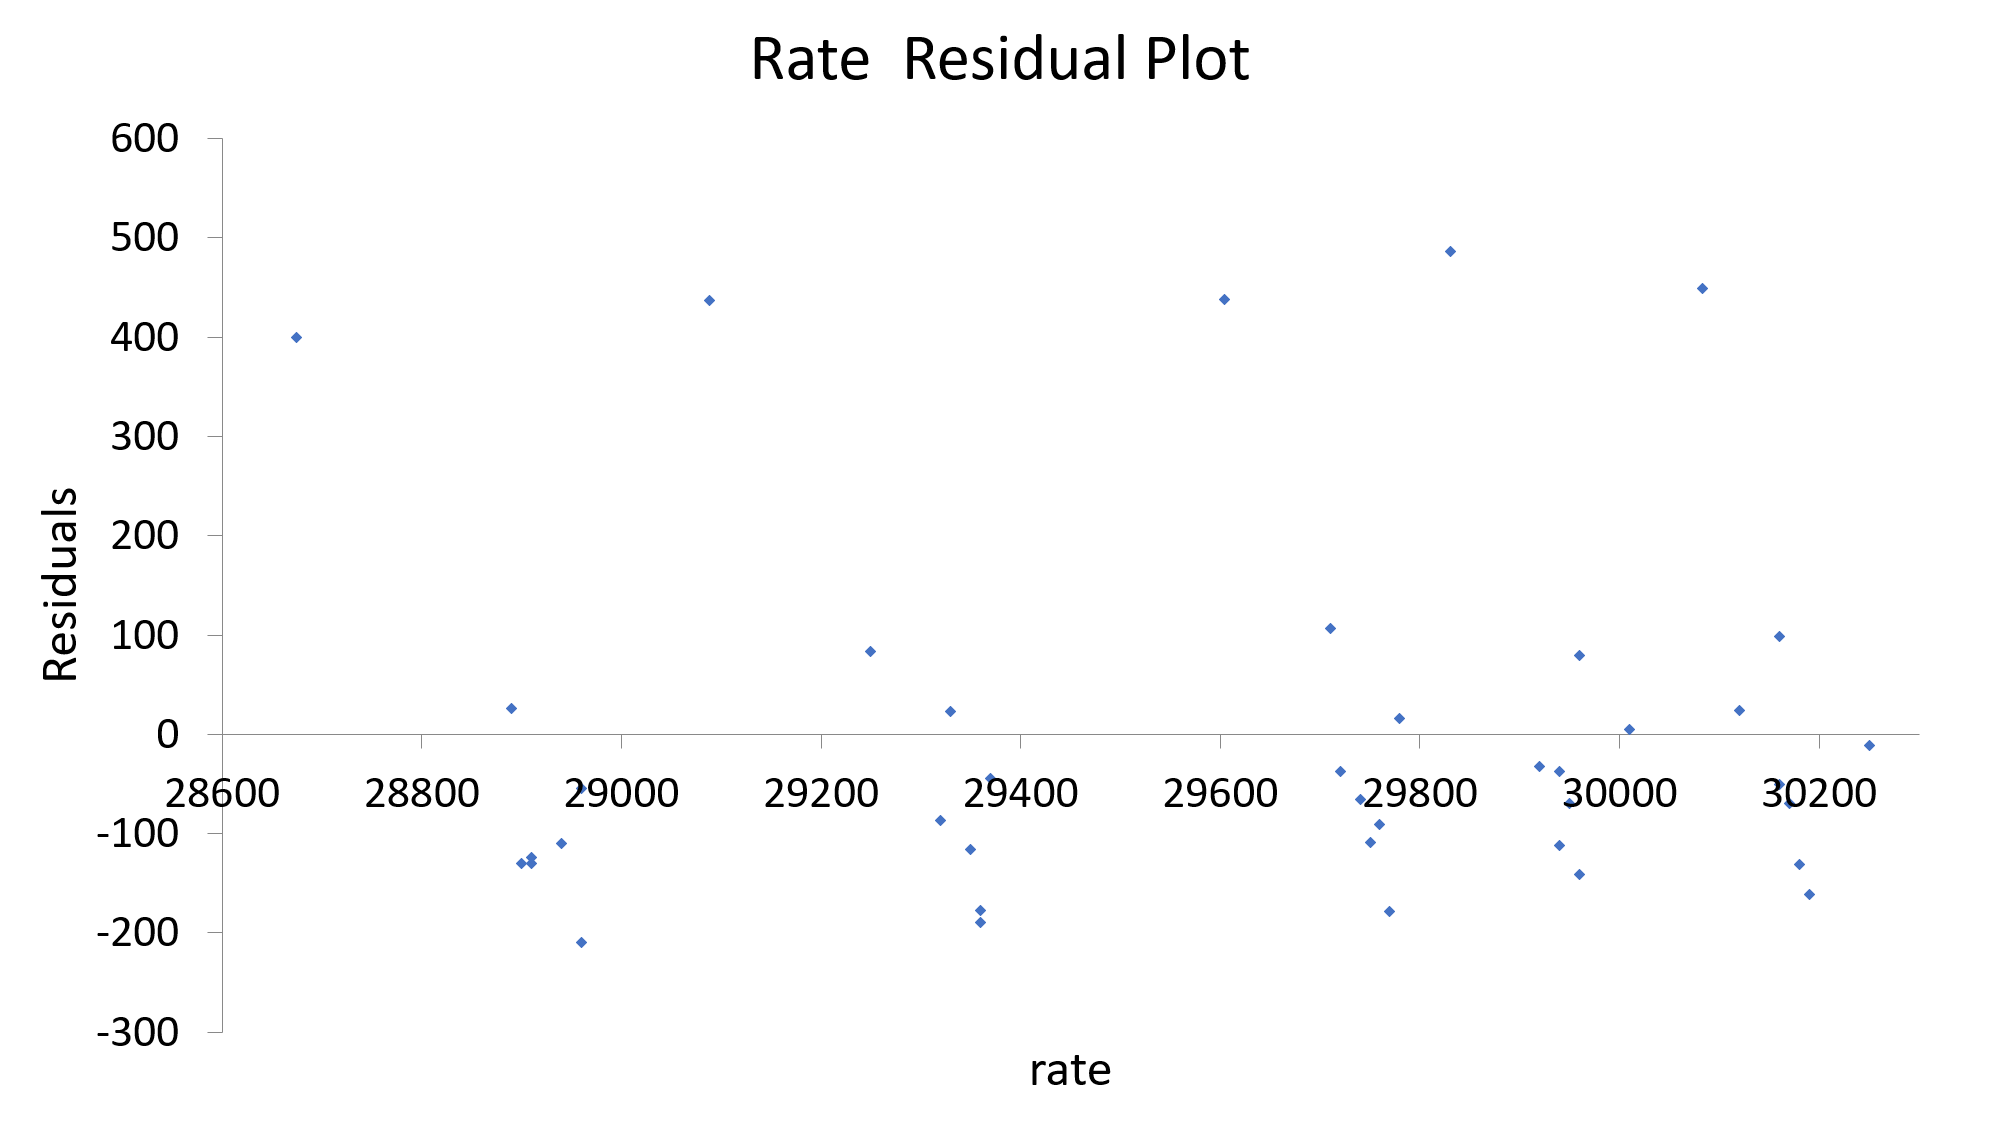
\includegraphics[width=\textwidth]{rateresidual.png}
 \caption{INSERT}
 % \label{q6}
\end{figure}
The residuals appear randomly scattered about the horizontal 0 line.
Additionally, we observe that the Normal Probability plot below
very closely represents a straight line, so the normality assumption for the
residuals does seem appropriate.
\todo{is it because there is a straight line, or is there a better explanation like the residuals being scattered about 0?}
\todo{do the assumptions hold?}

\begin{figure}[H]
 \centering
 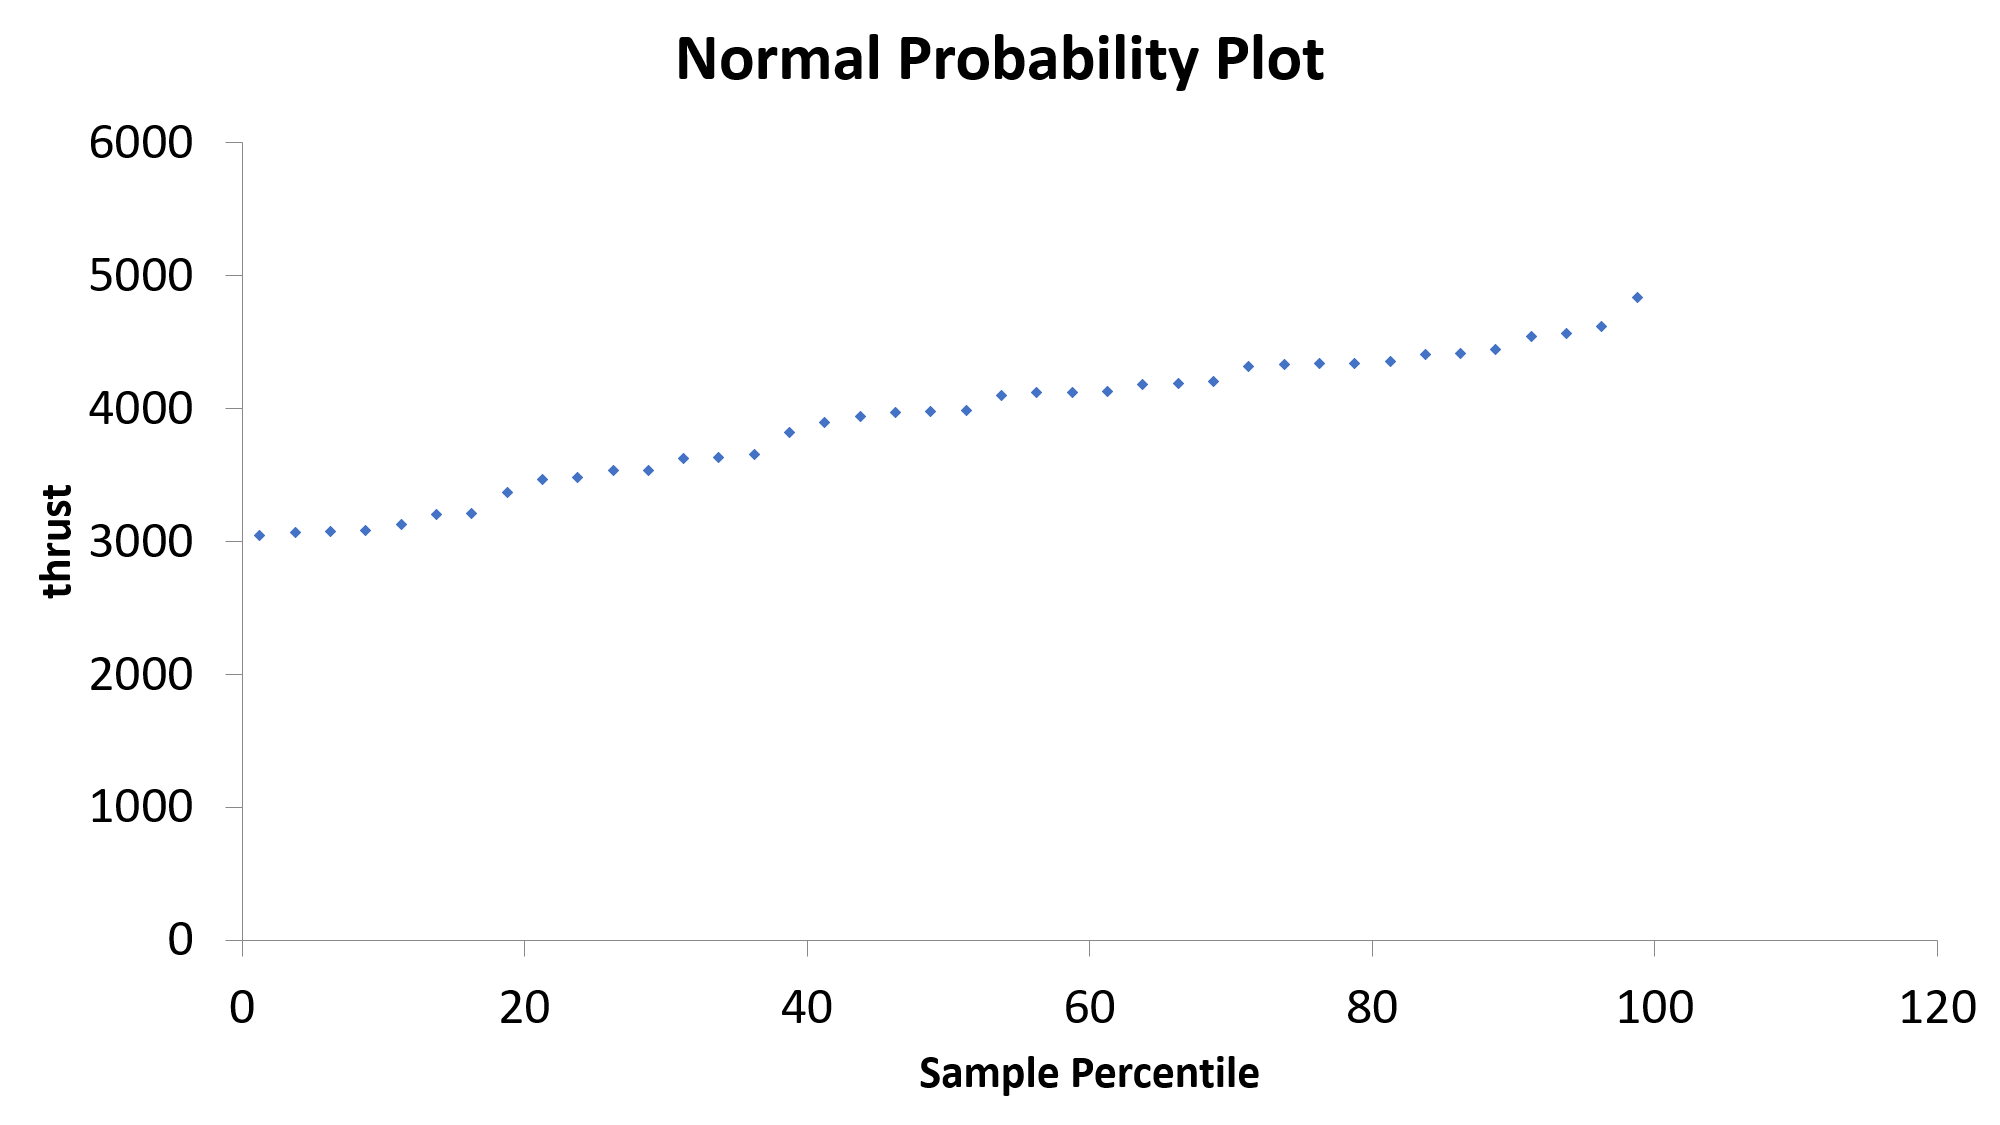
\includegraphics[width=\textwidth]{normalplot.png}
 \caption{INSERT}
 % \label{q6}
\end{figure}

\section{}
% OUTPUT: Regression output. Optional.

\subsection{}
% Equation of regression with coefficient values. Determine
% influential points from scatter plot in Q1. Determine outlier residuals from residual plot.

Using the regression tool in Excel, we find $\beta_0=-6643.268654$, and
$\beta_1=6.384931687$.
So, Equation \ref{model} becomes
$$ thrust = -6643.268654 + 6.384931687 \times (extemp) + \epsilon$$
\todo{should $\epsilon$ be in this equation?}

From the scatterplot in Figure \ref{extempthrust}, there don't seem to be any
influential points which are far away from the rest of the data. Similarly, there
are no obvious outliers in the residual plot.

\subsection{}
The estimate of the model standard deviation is:
$$s = 250.5362661$$
\todo{compare to average? wtf???}

\subsection{}
% Percent of variation? What might explain variation?

The percentage of the variation in thrust which is explained by the fuel flow rate
is the $R^2$ value.
$$R^2 = 0.759847831 \approx 75.98\%$$
The other predictor variables rate and ambtemp may explain the remaining variation
(probably the rate variable moreso than the ambtemp variable).
% \todo{What other possible predictor variables may explain the remaining variation?}

\subsection{}
% Hypotheses? What kind of test can you use? Values of test
% statistics? P-value? Null distribution? Conclusion?

Let the null hypothesis be that the fuel flow rate does not have any value in explaining the thrust:
$$ H_0: \beta_1 =0 \quad vs. \quad H_A: \beta_1 \neq 0 $$
The distribution of the test statistic follows a null dustribution.
Using Excel, we find that
$$F_0 = 10.9650813 \sim F_{39-2}^{1}$$
\todo{idk what I'm doing wrong here}
The p-value is
$$p= \SI{2.48143e-13}{} $$
Because the p-value obtained is extremely small, we reject $H_0$. i.e. the data strongly suggests that there is a relationship between the external temperature and the thrust.

\setcounter{subsection}{6}
\subsection{}
% OUTPUT: Residual Plot. Interpret the plot. Are the assumptions met?

\begin{figure}[H]
 \centering
 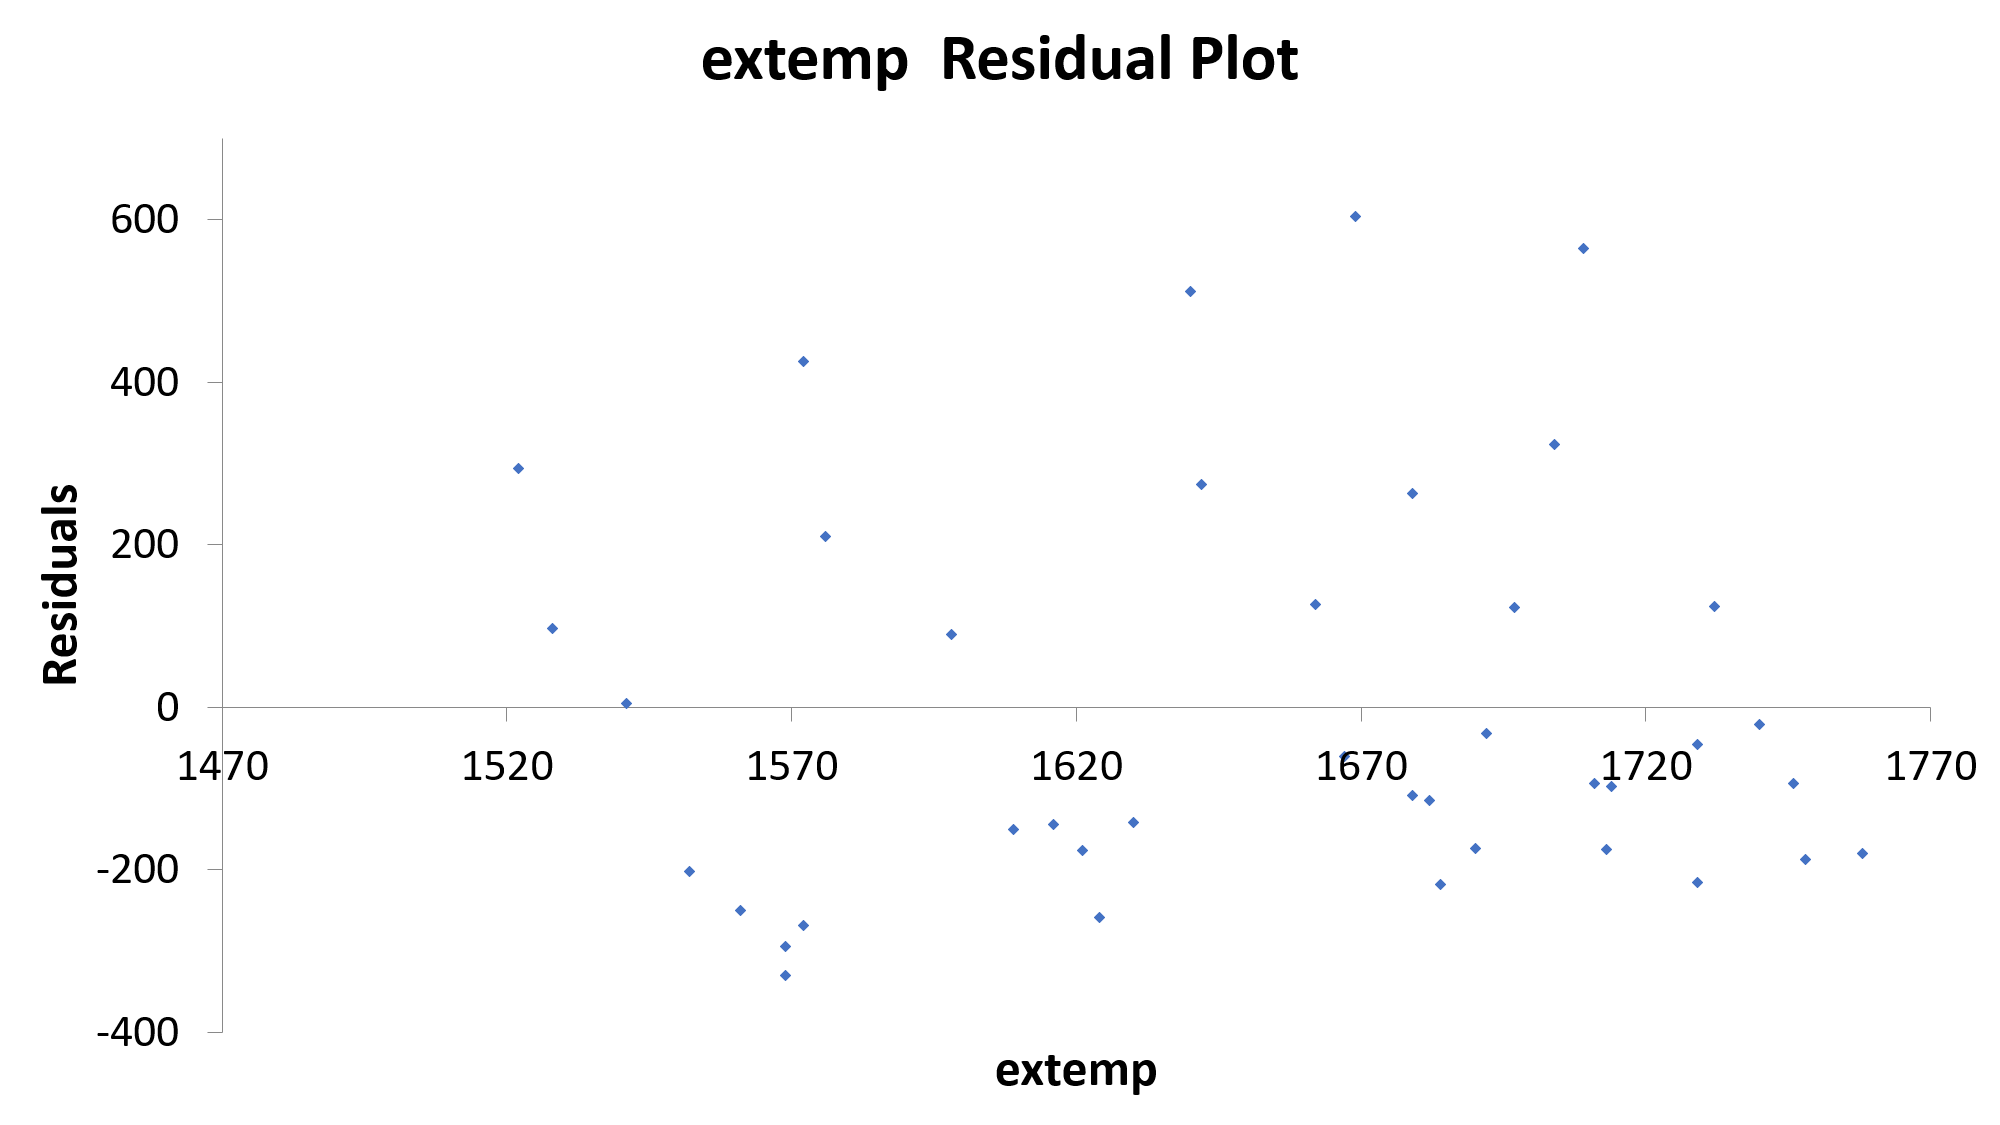
\includegraphics[width=\textwidth]{extempresidual.png}
 \caption{INSERT}
 % \label{q6}
\end{figure}
The residuals appear randomly scattered about the horizontal 0 line.
Additionally, we observe that the Normal Probability plot below
very closely represents a straight line, so the normality assumption for the
residuals does seem appropriate.
\todo{is it because there is a straight line, or is there a better explanation like the residuals being scattered about 0?}
\todo{do the assumptions hold?}

\begin{figure}[H]
 \centering
 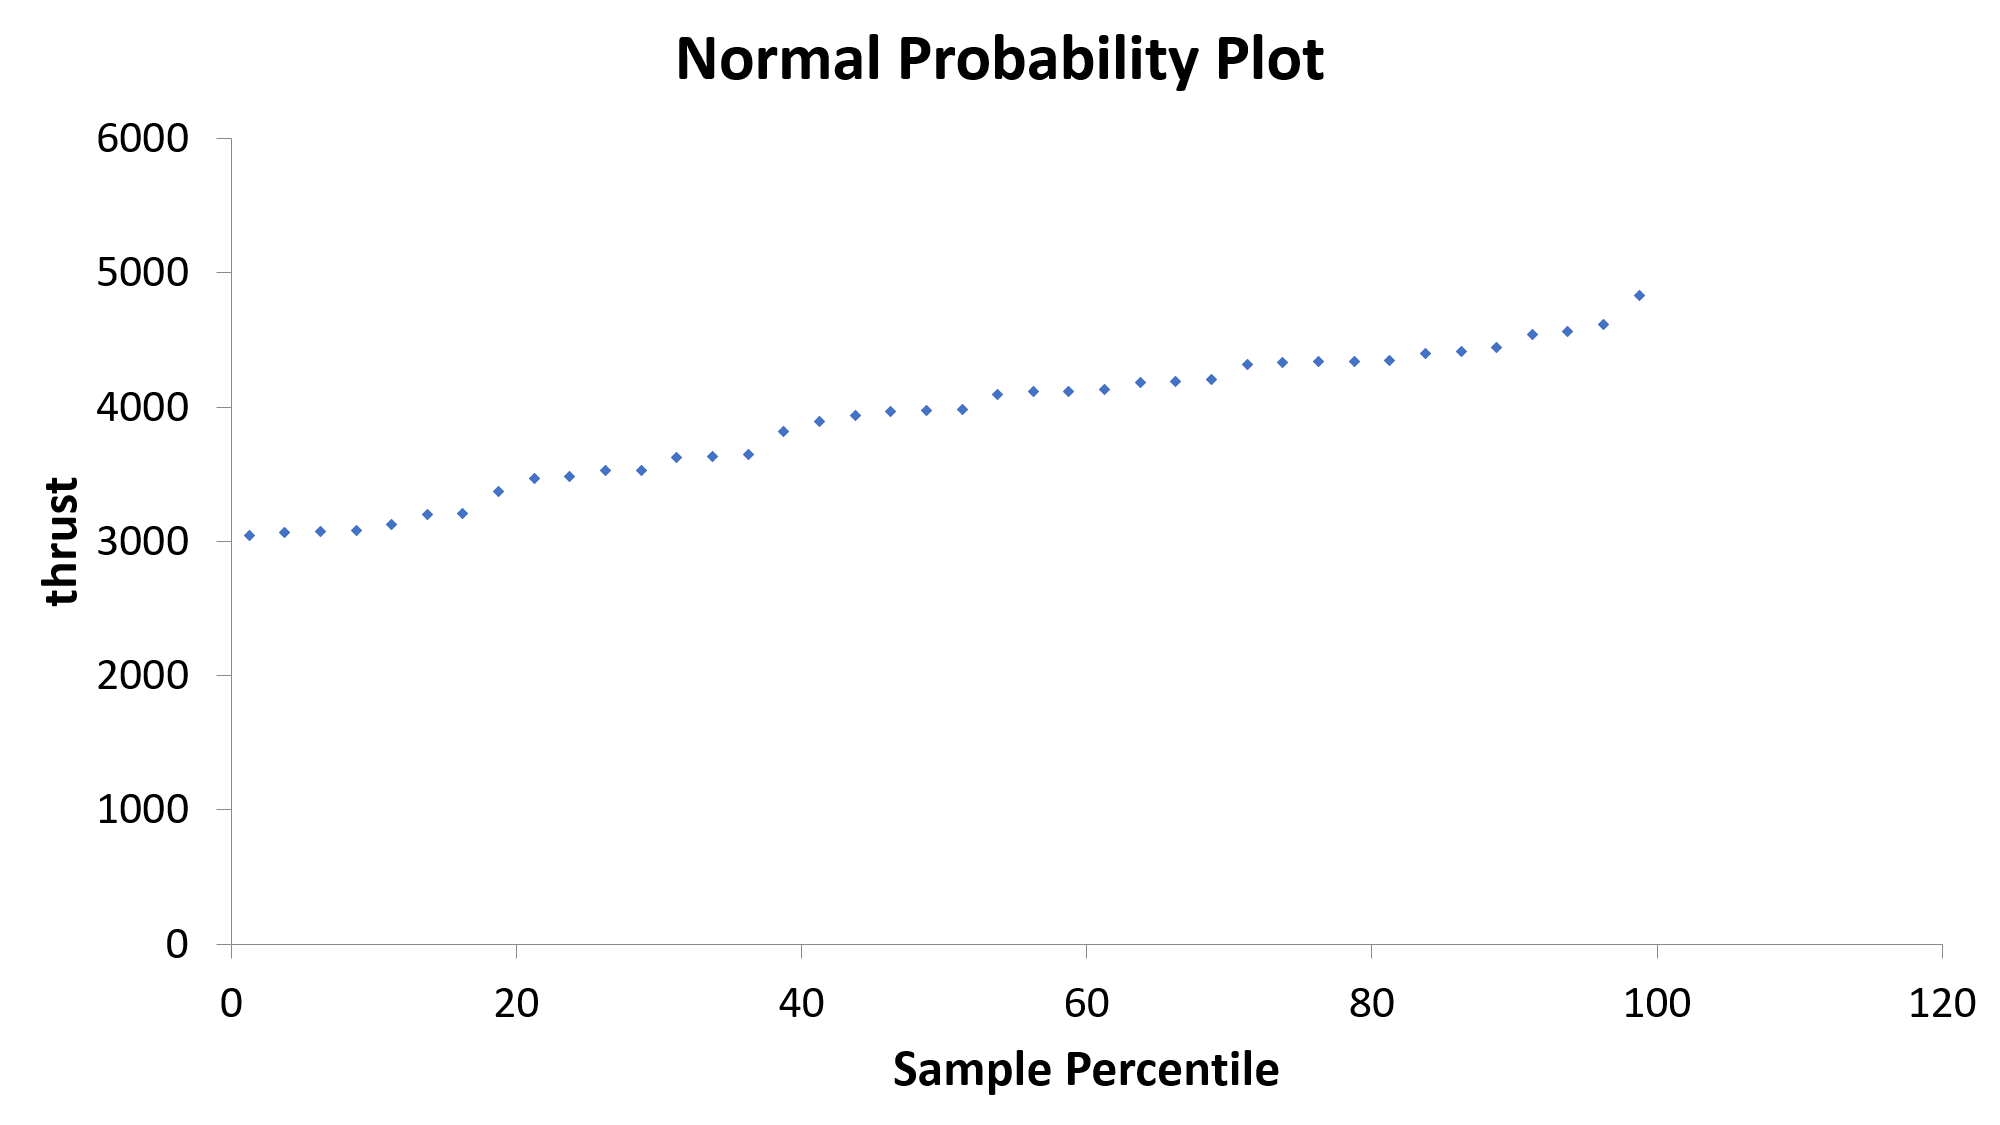
\includegraphics[width=\textwidth]{normalplot2.png}
 \caption{INSERT}
 % \label{q6}
\end{figure}

\section{}
% What’s the best predictor? S = model standard deviation

\begin{table}[H]
 \centering
 \begin{tabular}{|c|c|c|c|c|}
  \hline
  Thrust vs. & $R^2$       & s           & t-statistic & p-value            \\ \hline
  Rate       & 0.862655506 & 189.466735  & 15.44915999 & \SI{5.72762e-18}{} \\ \hline
  Extemp     & 0.759847831 & 250.5362661 & 10.9650813  & \SI{2.48143e-13}{} \\ \hline
 \end{tabular}
 \caption{My caption}
 \label{q6}
\end{table}

The fuel flow rate appears to be the best predictor of thrust. It has a stronger
correlation (larger $R^2$), and it also accounts for a larger percentage of the
variation in thrust. It also has a smaller standard error, and a much smaller
p-value.


\newpage
\thispagestyle{empty}
\begin{figure}
 \centering
 
\includegraphics[width=\textwidth]{correlation.png}
 % \caption{---}
 \label{xkcd}
\end{figure}

\end{document}
